% !TeX program = lualatex
% !TeX root = main.tex

\chapter{Clustering and combined distances}
\emph{%
This chapter covers the basics of clustering. It first describes the used clustering algorithm DBSCAN, followed by the distance metrics for geographical distance and text distance. At last the combined distance metric is presented.
}\label{chap:cluster}

\section{Cluster analysis}
As introduced in chapter~\ref{chap:topics}, \emph{cluster analysis} is the task of grouping a set of objects $\{o_1, \dots, o_n\}$ based on similarity, which is expressed as a distance function $f: o_i \times o_j \rightarrow \mathbb{R}$. There are many different clustering algorithms\cite{Berkhin2006}, each with there own problems and advantages. Two often used concepts are hierarchical clustering, and k-means.

\subsubsection*{Hierarchical clustering}
Hierarchical clustering builds a hierarchy,\,/\,tree of documents called dendrogram. The cluster set can be retrieved for example by choosing a tree level; then all child nodes which have the same parent at this level are together in a cluster. The dendrogram can be computed in two ways: 
    
Agglomerative, which starts with each document as its own cluster, and then joins them successively (\enquote{bottom up} approach). Or divisive, which starts with one giant cluster, and then performs splits recursively, until every document is alone (\emph{top down} approach).

The definition of a distance between the clusters, based on which all joining\,/\,splitting happens, is called link criterion. There are many different ones; two obvious examples are complete linkage clustering $\max \{f(a,b): a \in A, b \in B\}$ and single-linkage clustering $\min \{f(a,b): a \in A, b \in B\}$. 

A great problem with using hierarchical clustering is the complexity of at least $O(n^2)$, especially considering the big datasets used in this thesis.

\subsubsection*{k-means}
k-means clusters objects into $n$ clusters. At the beginning, $n$ points are chosen as initial cluster centroids. Then each point is being assigned to the nearest cluster center. After that new cluster centroids are calculated, usually the mean of all points assigned to it. Point assignment and center recalculation is done until the centroids are stable.

The k-means algorithm is relatively simple and easy to adopt to new domains and tasks, which explains its popularity. Finding a global optimal solution is considered NP-hard, but there are approximations with polynomial complexity, or solutions for \enquote{good enough} results by carefully choosing the initial cluster centroids.

Problems with k-means are the initial choice of the number of clusters and, depending on the distance function, the weakness in finding arbitrary shaped clusters.

\vspace{1em}
\noindent
This leads directly to the used clustering algorithm, which does not have the problems of the two ones described above.

\section{DBSCAN}
DBSCAN (density-based spatial clustering of applications with noise) by \textcite{Ester1996} is a density-based clustering algorithm. It is able to detect arbitrary shaped clusters and does not need the number of clusters beforehand. It performs also well with a complexity of $O(n \log n)$, which makes it usable for big data sets, and it has a notion of noise; of points which are so different they belong to no cluster.

Density describes the amount of elements in a given area. DBSCAN defines this as the $\epsilon$- or $eps$-neighbourhood $N_{eps}(p)$ of a point $p$, which are all points $q$ with distance $d(p, q)$ smaller $eps$.
%
\begin{align*}
N_{eps}(p) &= {q \in D | d(p,q) \leq eps}
\end{align*}
%
Furthermore DBSCAN differentiates between two kinds of points: 
%
\begin{align*}
|N_{eps}(p)| \geq minPts &\rightarrow core\\
else &\rightarrow border
\end{align*}
%
$core$ points have at least $minPts$ in their $eps$ neighbourhood, $border$ points have less.

Density as the amount of elements in a given area is naturally described by $N_{eps}$ and $minPts$. These dense neighbourhoods of core points are then connected through their density. A point $p$ is directly density reachable from $q$, if $p \in N_{eps}(q)$ and $q$ is $core$ point. Directly density reachability is asymmetric if one of the two points is a $border$ point.

Extending on directly density reachability is the definition of density reachability. A point $p$ is density reachable from a point $q$, if there is a path of points $p, p_1, \dots, p_n, q$, so that $p_{i+1}$ is directly density reachable from $p_i$. This is again asymmetric, if one of the two points is a $border$ point.

Because two $border$ points can not density reach each other, the notion of density connectivity is introduced, which is symmetric. Two points $q$ and $p$ are density connected, if there is a third point $k$ that can reach both $q$ and $p$ through density reachability. Clusters and noise are now defined based on density connectivity. 

A cluster $c$ is a subset of documents of a dataset $D$ with regard to $eps$ and $minPts$, so that for all $core$ points $p, q \in c$ are density reachable to each other, and all $border$ points are density connected to $core$ points. If $c_1, \dots, c_n$ are all clusters of $D$ (always regarding $eps$ and $minPts$), then $noise$ are all those points not belonging to any cluster.

Every cluster has a size of at least $minPts$. DBSCAN has stable results regarding $core$ points; they are always in the same cluster, regardless of the order of processing, because they are always density reachable. $border$ points can change their affiliation of a cluster, because they could be reached by different $core$ points, who could belong to different cluster.

\newpage
\subsection{Algorithm}
As previously seen, DBSCAN requires the following two parameters:

\begin{enumerate}
\item $eps$ (eps), which defines the minimum distance of $p$ to all points in $N_{eps}(p)$, and
\item $minPts$, which defines the minimum number of points needed inside $N_{eps}(p)$ for $p$ to be a core point.
\end{enumerate}

A pseudo code of the algorithm can be found in listing~\ref{dbscan}. DBSCAN starts at an unvisited random point $p$ and checks if $|N_{eps}(p)| \geq minPts$. If this requirement is not met, $p$ will be marked as noise. $p$ could later be reached by another point and thus clustered being a border point. If $|N_{eps}(p)| \geq minPts$ is true a new cluster $C$ is created. 

Now every point $q$ in $N_{eps}(p)$ is added to the cluster $C$ (if not already in another cluster as a border point). Iteratively the size of every $N_{eps}(q)$ is checked and points added to $N$ for further investigation until $N$ is empty.

At last the circle starts again with another random, unvisited point, until all points are visited.

\begin{algorithm}[tb]
\caption{DBSCAN algorithm}\label{dbscan}
\begin{algorithmic}[1]
\Function{DBSCAN}{D, $eps$, $MinPts$}
\ForAll{p $\in$ D, p \textbf{not marked as} VISITED}
	\State \textbf{mark} p \textbf{as} VISITED
	\State N \gets D.regionQuery(P, $eps$)
	\If{\Call{sizeof}{N} $\geq MinPts$}
		\State C \gets next cluster
		\State \Call{expandCluster}{p, N, C, $eps$, $MinPts$}
	\Else		
		\State \textbf{mark} p \textbf{as} NOISE
	\EndIf
\EndFor
\EndFunction
\Statex
\Function{expandCluster}{p, N, C, $eps$, $MinPts$}
\State \textbf{add} p \textbf{to} cluster C
\ForAll{q $\in$ N, q \textbf{not marked as} VISITED}
	\State \textbf{mark} q \textbf{as} VISITED
	\State M \gets \Call{regionQuery}{q, $eps$}
	\If{\Call{sizeof}{M} $\geq MinPts$}
		\State N \gets N $\cup$ M
	\EndIf
	\If{q is not yet member of any cluster}
		\State \textbf{add} q \textbf{to} cluster C
	\EndIf
\EndFor
\EndFunction
\Statex
\Function{regionQuery}{p, $eps$}
\State \Return all points within $N_{eps}(\text{p})$
\EndFunction
\end{algorithmic}
\end{algorithm}

The algorithm performs basically a $regionQuery$ for every point in the dataset in order to get all $eps$ neighbourhoods. Hence the complexity of DBSCAN depends on the complexity for this $regionQuery$: $O(n \, \, O(regionQuery))$. A very simple $regionQuery$ can be a linear search over all other points, resulting in an overall complexity of $O(n^2)$, which is effectively a distance matrix. Such a distance matrix can be precomputed for subsequent execution on the same dataset, but this would require $O(n^2)$ memory. Usually a better strategy involves the usage of an appropriate index structure, for example R-trees or kd-trees, which work very well for spatial data. Most of these index structures have an average neighbourhood search complexity of $O(\log n)$, with leads to an overall average complexity of $O(n \log n)$ for DBSCAN.

Datasets with very various densities can be problematic, because the two parameters $eps$ and $MinPts$ only describe one density threshold. Hence DBSCAN is unable to detect a cluster within another cluster with different density, as long as both are denser than the threshold. Also the used distance\,/\,neighbourhood function must be chosen carefully; the so called \enquote{curse of dimensionality} can render any $eps$\,/\,$MinPts$ combination useless due to high dimensional data with an unfitting distance function.

DBSCAN does not require the number of cluster beforehand. This is especially useful if there is no viable visualization or there is no clue for guessing. Arbitrary shaped clusters can be found, and points have not to be clustered at all, if they are too different (noise). Building clusters depends only on the distances between points; in fact, they depend only on the $eps$-neighbourhood queries, which enables the usage of a wide variety of data and distance\,/\,neighbourhood functions.


\section{Distance Metrics}\label{sec:distance}
Besides the choice of the two parameters for DBSCAN, the underlying distance function is of great importance. This distance function has to follow some rules in order to be useful in DBSCAN. It has to obey the following first two rules from the definition of a metric (all rules given for completeness, and because most useful distance functions are metrics after all).

A metric on a set $X$ is a function (called the distance function or simply distance) $d : X × X → R$. For all $x, y, z$ in $X$, this function is required to satisfy the following conditions:
\begin{enumerate}
\item $d(x, y) \geq 0$ (non-negativity)%, or separation axiom)
\item $d(x, y) = d(y, x)$ (symmetry)
\item $d(x, y) = 0$ if and only if $x = y$ %(identity of indiscernibles, or coincidence axiom)
\item $d(x, z) \leq d(x, y) + d(y, z)$ (triangle inequality)%subadditivity
\end{enumerate}

%\subsection{Time distance}
%The distance between two timestamps $t_1$ and $t_2$ is the time passed between those two events; the timespan between them:
%\begin{align*}
%d^{time}_{12} = |t_1 - t_2|
%\end{align*}
%The interval of $d^{time}$ is $[0, t_{max}-t_{min}]$.

\subsection{Text distance}
There are many different distance metrics to measure the (dis)similarity between texts respectively documents\cite{Huang2008}. Depending on the lengths of the text and the additional tasks upon them (searching, ranking), it is important to use an appropriate metric.

The distance metric used in this thesis for texts is the Jaccard distance\cite{Manning2009} on top of bigrams of the texts, which has been effectively used for clustering text\cite{Huang2008}. A bigram is the set of all adjacent two-letter fragments of a text. For example the word $distance$ has the following bigram: $(di, is, st, ta, an, nc, ce)$. The Jaccard index $J$ is defined as the size of the intersection divided by the size of the union of two bigrams $A$ and $B$. This measures the similarity of the two sets. The Jaccard distance $d_{text}$ is then calculated by subtraction of $J$ from $1$:
%
\enlargethispage{\baselineskip}
\begin{align}
J(A, B) &= \frac{|A \cap B|}{|A \cup B|}\notag\\
d_{text}(A, B) &= 1 - J(A, B) = \frac{|A \cup B| - |A \cap B|}{|A \cup B|}
\end{align}
The interval of $d_{text}$ is $[0, 1]$.

\subsubsection{Example}
The text distance between the words \emph{distance} and \emph{maintenance} has to be calculated. The sets $A$ and $B$ contain the bigrams:
\begin{align*}
A &= di, is, st, ta, an, nc, ce\\
B &= ma, ai, in, nt, te, en, na, an, nc, ce
\end{align*}
%
The intersection and union of $A$ and $B$ is as follows
\begin{align*}
|A \cap B| &= |an, nc, ce| = 3\\ %intersection
|A \cup B| &= |di, is, st, ta, ma, ai, in, nt, te, en, na, an, nc, ce| = 14 %union
\end{align*}
%
which leads to the final distance
\begin{align*}
d_{text} &= 1 - \frac{3}{14} \approx 0.786
\end{align*}

\subsection{Location distance}
The given GPS data (Latitude ($lat$)\,/\,Longitude($lon$)-pairs) are locations on the earth; positions on top of a (rather non-uniform) ellipsoid. The optimal way of computing the distance between two points would be in calculating the distance on top of this ellipsoid (great-circle distance).

But this is time-consuming and ugly to handle. Another way is to project the coordinates onto a plane and calculate an approximation with basic trigonometry and euclidean distances. This can be done thinking of the center of the earth as one corner of a triangle, and the two locations (whose distance from one another is wanted) as the other two corners, resulting in the following formula, which is sometimes called planar projection:

\begin{align*}
x &= (A_{lon} - B_{lon}) * cos(\frac{A_{lat} + B_{lat}}{2})\\
y &= (A_{lat} - B_{lat})\\
d &= R \, \frac{\pi}{180} \, \sqrt{x^2 + y^2}
\end{align*}
%
$R$ is \enquote{the} radius of the earth, which is 6373~km in this thesis. The factor $cos(\frac{A_{lat} + B_{lat}}{2})$ is used to correct the wide for one longitude degree, which \enquote{grows tighter} the nearer it is to the poles. This factor will be omitted for practical reasons (usage of a spatial index for fast neighbour queries), as well as $R$ and $\frac{pi}{180}$, which are not needed for just comparing distances.

\begin{align}
d_{loc}(A, B) &= \sqrt{(A_{lat} - B_{lat})² + (A_{lon} - B_{lon})²}
\end{align}
%
This euclidean distance is good enough for comparing distances. For example the great-circle distance between Berlin ($lat$: 52.66, $lon$: 13.51) and Bonn ($lat$: 50.74, $lon$: 7.10) is 739.52~km, while the euclidean distance is 6.69° or 744.26~km.

%\todo{comparison great-circle vs euclidean}

%>>> from pyproj import Geod
%>>> g = Geod(ellps='WGS84')
%>>> g.inv(52.655561,13.507462, 50.739932,7.10392)
%(-163.31731230887556, 16.339412526021903, 738694.1895019277)
%Berlin to Bonn
%great-circle distance 738.69~km
%>>> from math import sqrt
%>>> sqrt(pow((52.655561- 50.739932),2) + pow((13.5 - 7.10392),2))
%6.676786190379395
%>>> sqrt(pow((52.655561- 50.739932),2) + pow((13.5 - 7.10392),2)) * 0.017453292519943295769236907684886 * 6372797.560856
%742634.2238470017
%euclidean 742.63~km

%\begin{wrapfigure}{r}{0.40\textwidth}
%  \begin{center}
%    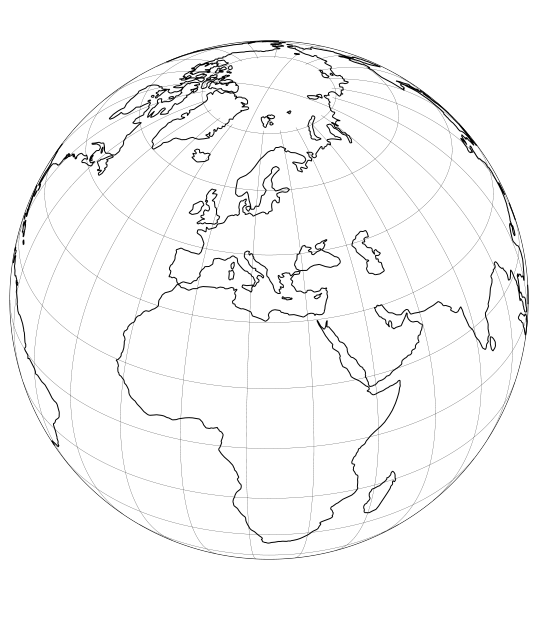
\includegraphics[width=0.38\textwidth]{pix/map_projection}
%  \end{center}
%  \caption{Globe with longitude and latitude lines\protect\footnotemark}
%\end{wrapfigure}

%\footnotetext{\url{http://kartograph.org/showcase/projections}}Locations are usually given in longitude\,/\,latitude-coordinates. This coordinate system divides the earth horizontally in 180 equal parts called latitude, which are parallel to each other. The north pole is 90°, the equator 0° and the south pole -90°.

%Longitude are called the 360 parts slicing the earth vertically. Those slices are not parallel; they start each at the north pole and end at the south pole.

%The earth is a rather non-uniform ellipsoid, hence each distance between two points is no straight line, but a path on a sphere at best. Distances on the surface of a sphere are called great-circle distances. Using euclidean distance is therefore prone to be more unprecise the greater the two points are afar and the greater the latitude gets.

%There are now three options depending the location distance measure:
%\begin{enumerate}
%\item Great-circle distance: precise, but slow to compute and no index-support.
%\item Euclidean distance: very fast to compute and index-support, but very inaccurate.
%\item Combination of both: use unprecise euclidean for nearest neighbour queries to reduce the possible candidates, the calculate the accurate distances with a great-circle distance.
%\item (alternative: dimension reduction for a projection of lat\,/\,lon to euclidean distances while preserving the distances)
%\end{enumerate}
 
%\section{Definitions}
%\begin{tabular}{ll}
%$d^n_{ij}$ & distance of type $n$ from $i$ to $j$\\
%\end{tabular}

\subsection{Combining the distance metrics}
After introducing the two fundamental distance metrics for text and location distances, they are joined in a linear combination in the form $\alpha \, d_{loc} + \beta \, d_{text} = d_{com}$. Of course, additional distance metrics could also be joined in the same linear fashion.

$\alpha$ and $\beta$ could be simple weights, but because the intervals of the metrics are different, they should also incorporate a way to align the distances. Thus, $\alpha$ and $\beta$ each consist of a weight $w$ and a normalisation factor $eps$. 

\begin{align}
d_{com} &= \alpha \,\, d_{loc} + \beta \,\, d_{text}\notag\\
d_{com} &= \frac{w_{loc}}{eps_{loc}} \, d_{loc} + \frac{w_{text}}{eps_{text}} \, d_{text}\\
\sum w &= 1 \notag
\end{align}
%
The normalization factor is called $eps$, because it has the same effect as the DBSCAN parameter $eps$, if one weight is set to 1 as well as DBSCAN $eps$:
\begin{align*}
1 &= \frac{1}{eps_{loc}} \, d_{loc} + \frac{0}{eps_{text}} \, d_{text}\\
&= \frac{1}{eps_{loc}} \, d_{loc}\\
d_{loc} &= eps_{loc}
\end{align*}
%
With this natural relation of these values, it is easy to understand the meaning of the normalization and finding usable values is much easier.